\documentclass{standalone}
\usepackage{tikz}
\usetikzlibrary{patterns, positioning}
\usetikzlibrary{shapes.misc}
\usepackage[outline]{contour}
\contourlength{1.5pt} 


\begin{document}
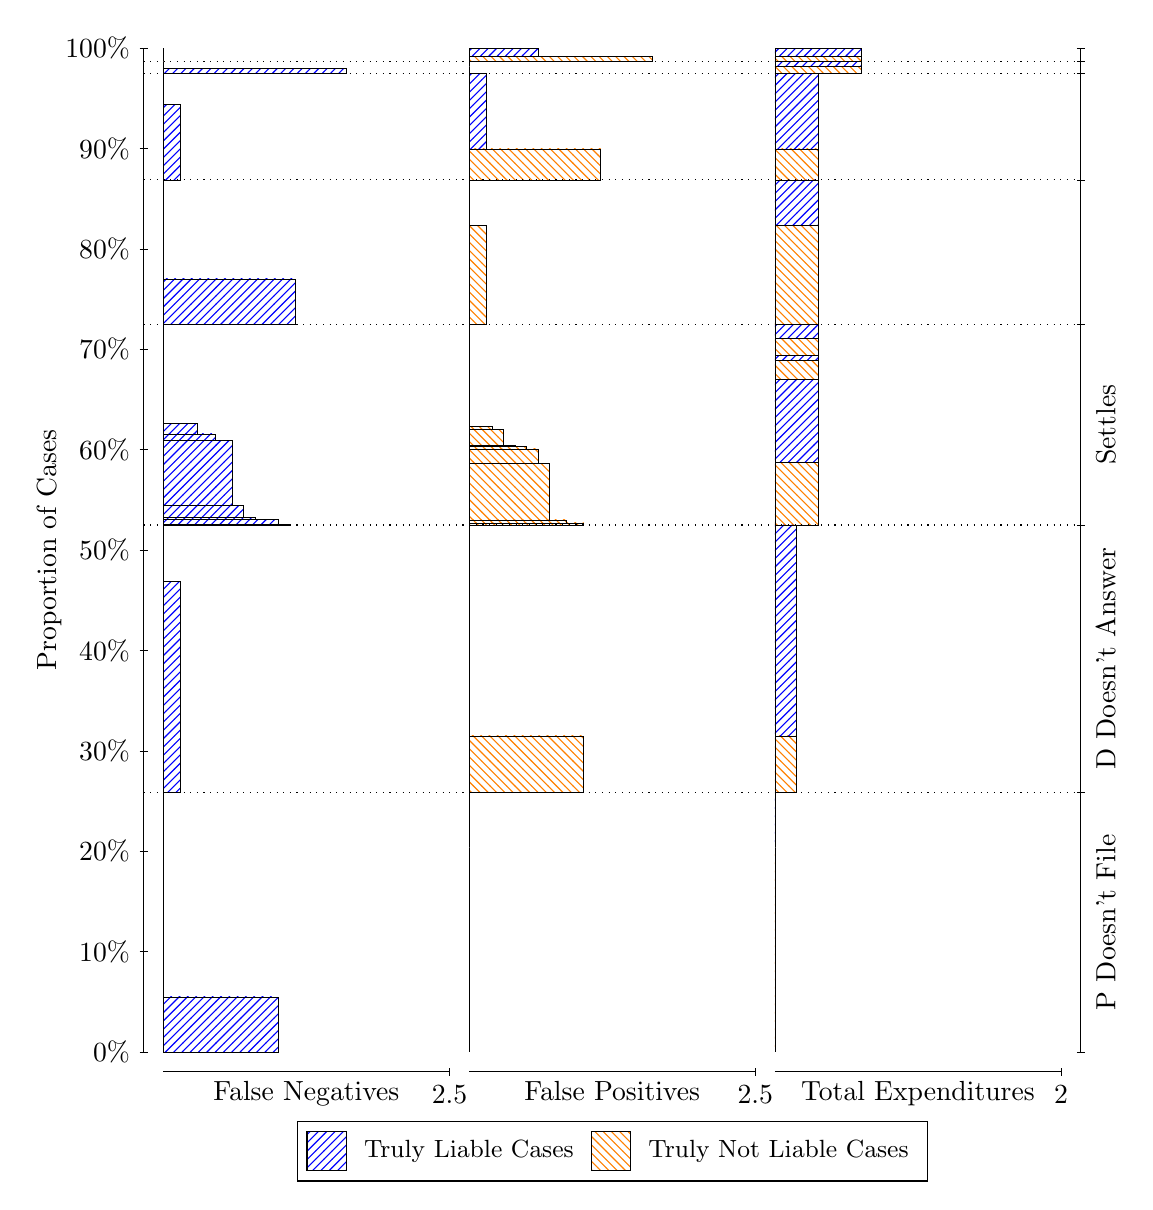
\begin{tikzpicture}
\draw[black, very thin] (1.5,1.75) -- (1.5,14.5);
\node[rotate=90, text=black, anchor=center] at (0.3, 8.125) {Proportion of Cases};
\draw[black, very thin] (1.45,1.75) -- (1.55,1.75);
\node[text=black, anchor=east] at (1.45, 1.75) {0\%};
\draw[black, very thin] (1.45,3.025) -- (1.55,3.025);
\node[text=black, anchor=east] at (1.45, 3.025) {10\%};
\draw[black, very thin] (1.45,4.3) -- (1.55,4.3);
\node[text=black, anchor=east] at (1.45, 4.3) {20\%};
\draw[black, very thin] (1.45,5.575) -- (1.55,5.575);
\node[text=black, anchor=east] at (1.45, 5.575) {30\%};
\draw[black, very thin] (1.45,6.85) -- (1.55,6.85);
\node[text=black, anchor=east] at (1.45, 6.85) {40\%};
\draw[black, very thin] (1.45,8.125) -- (1.55,8.125);
\node[text=black, anchor=east] at (1.45, 8.125) {50\%};
\draw[black, very thin] (1.45,9.4) -- (1.55,9.4);
\node[text=black, anchor=east] at (1.45, 9.4) {60\%};
\draw[black, very thin] (1.45,10.675) -- (1.55,10.675);
\node[text=black, anchor=east] at (1.45, 10.675) {70\%};
\draw[black, very thin] (1.45,11.95) -- (1.55,11.95);
\node[text=black, anchor=east] at (1.45, 11.95) {80\%};
\draw[black, very thin] (1.45,13.225) -- (1.55,13.225);
\node[text=black, anchor=east] at (1.45, 13.225) {90\%};
\draw[black, very thin] (1.45,14.5) -- (1.55,14.5);
\node[text=black, anchor=east] at (1.45, 14.5) {100\%};

\draw[black, very thin] (13.4,1.75) -- (13.4,14.5);
\draw[black, very thin] (13.35,1.75) -- (13.45,1.75);
\node[anchor=west] at (13.35, 1.75) {};
\draw[black, very thin] (13.35,5.0449) -- (13.45,5.0449);
\node[anchor=west] at (13.35, 5.0449) {};
\draw[black, very thin] (13.35,8.4431) -- (13.45,8.4431);
\node[anchor=west] at (13.35, 8.4431) {};
\draw[black, very thin] (13.35,10.989) -- (13.45,10.989);
\node[anchor=west] at (13.35, 10.989) {};
\draw[black, very thin] (13.35,12.825) -- (13.45,12.825);
\node[anchor=west] at (13.35, 12.825) {};
\draw[black, very thin] (13.35,14.18) -- (13.45,14.18);
\node[anchor=west] at (13.35, 14.18) {};
\draw[black, very thin] (13.35,14.33) -- (13.45,14.33);
\node[anchor=west] at (13.35, 14.33) {};
\draw[black, very thin] (13.35,14.5) -- (13.45,14.5);
\node[anchor=west] at (13.35, 14.5) {};

\draw[black, very thin, pattern color=blue, pattern=north east lines] (1.75,1.75) rectangle (3.2033,2.4503);
\draw[black, very thin, pattern color=orange, pattern=north west lines] (1.75,2.4503) rectangle (1.75,5.0449);
\draw[black, very thin, pattern color=blue, pattern=north east lines] (1.75,5.0449) rectangle (1.968,7.7224);
\draw[black, very thin, pattern color=orange, pattern=north west lines] (1.75,7.7224) rectangle (1.75,8.4431);
\draw[black, very thin, pattern color=blue, pattern=north east lines] (1.75,8.4431) rectangle (3.3487,8.454);
\draw[black, very thin, pattern color=blue, pattern=north east lines] (1.75,8.454) rectangle (3.2033,8.5097);
\draw[black, very thin, pattern color=blue, pattern=north east lines] (1.75,8.5097) rectangle (3.058,8.5183);
\draw[black, very thin, pattern color=blue, pattern=north east lines] (1.75,8.5183) rectangle (2.9127,8.5379);
\draw[black, very thin, pattern color=blue, pattern=north east lines] (1.75,8.5379) rectangle (2.7673,8.6955);
\draw[black, very thin, pattern color=blue, pattern=north east lines] (1.75,8.6955) rectangle (2.622,9.52);
\draw[black, very thin, pattern color=blue, pattern=north east lines] (1.75,9.52) rectangle (2.404,9.6006);
\draw[black, very thin, pattern color=blue, pattern=north east lines] (1.75,9.6006) rectangle (2.186,9.7331);
\draw[black, very thin, pattern color=orange, pattern=north west lines] (1.75,9.7331) rectangle (1.75,10.989);
\draw[black, very thin, pattern color=blue, pattern=north east lines] (1.75,10.989) rectangle (3.4213,11.569);
\draw[black, very thin, pattern color=orange, pattern=north west lines] (1.75,11.569) rectangle (1.75,12.825);
\draw[black, very thin, pattern color=blue, pattern=north east lines] (1.75,12.825) rectangle (1.968,13.785);
\draw[black, very thin, pattern color=orange, pattern=north west lines] (1.75,13.785) rectangle (1.75,14.18);
\draw[black, very thin, pattern color=blue, pattern=north east lines] (1.75,14.18) rectangle (4.0753,14.244);
\draw[black, very thin, pattern color=orange, pattern=north west lines] (1.75,14.244) rectangle (1.75,14.33);
\draw[black, very thin, pattern color=orange, pattern=north west lines] (1.75,14.33) rectangle (1.75,14.397);
\draw[black, very thin, pattern color=blue, pattern=north east lines] (1.75,14.397) rectangle (1.75,14.5);
\draw[black, very thin, pattern color=orange, pattern=north west lines] (5.6333,1.75) rectangle (5.6333,4.3446);
\draw[black, very thin, pattern color=blue, pattern=north east lines] (5.6333,4.3446) rectangle (5.6333,5.0449);
\draw[black, very thin, pattern color=orange, pattern=north west lines] (5.6333,5.0449) rectangle (7.0867,5.7656);
\draw[black, very thin, pattern color=blue, pattern=north east lines] (5.6333,5.7656) rectangle (5.6333,8.4431);
\draw[black, very thin, pattern color=orange, pattern=north west lines] (5.6333,8.4431) rectangle (7.0867,8.4702);
\draw[black, very thin, pattern color=orange, pattern=north west lines] (5.6333,8.4702) rectangle (6.8687,8.5085);
\draw[black, very thin, pattern color=orange, pattern=north west lines] (5.6333,8.5085) rectangle (6.6507,9.2233);
\draw[black, very thin, pattern color=orange, pattern=north west lines] (5.6333,9.2233) rectangle (6.5053,9.4101);
\draw[black, very thin, pattern color=orange, pattern=north west lines] (5.6333,9.4101) rectangle (6.36,9.4366);
\draw[black, very thin, pattern color=orange, pattern=north west lines] (5.6333,9.4366) rectangle (6.2147,9.454);
\draw[black, very thin, pattern color=orange, pattern=north west lines] (5.6333,9.454) rectangle (6.0693,9.6553);
\draw[black, very thin, pattern color=orange, pattern=north west lines] (5.6333,9.6553) rectangle (5.924,9.6991);
\draw[black, very thin, pattern color=blue, pattern=north east lines] (5.6333,9.6991) rectangle (5.6333,10.989);
\draw[black, very thin, pattern color=orange, pattern=north west lines] (5.6333,10.989) rectangle (5.8513,12.245);
\draw[black, very thin, pattern color=blue, pattern=north east lines] (5.6333,12.245) rectangle (5.6333,12.825);
\draw[black, very thin, pattern color=orange, pattern=north west lines] (5.6333,12.825) rectangle (7.3047,13.219);
\draw[black, very thin, pattern color=blue, pattern=north east lines] (5.6333,13.219) rectangle (5.8513,14.18);
\draw[black, very thin, pattern color=orange, pattern=north west lines] (5.6333,14.18) rectangle (5.6333,14.266);
\draw[black, very thin, pattern color=blue, pattern=north east lines] (5.6333,14.266) rectangle (5.6333,14.33);
\draw[black, very thin, pattern color=orange, pattern=north west lines] (5.6333,14.33) rectangle (7.9587,14.397);
\draw[black, very thin, pattern color=blue, pattern=north east lines] (5.6333,14.397) rectangle (6.5053,14.5);
\draw[black, very thin, pattern color=orange, pattern=north west lines] (9.5167,1.75) rectangle (9.5167,4.3446);
\draw[black, very thin, pattern color=blue, pattern=north east lines] (9.5167,4.3446) rectangle (9.5167,5.0449);
\draw[black, very thin, pattern color=orange, pattern=north west lines] (9.5167,5.0449) rectangle (9.7892,5.7656);
\draw[black, very thin, pattern color=blue, pattern=north east lines] (9.5167,5.7656) rectangle (9.7892,8.4431);
\draw[black, very thin, pattern color=orange, pattern=north west lines] (9.5167,8.4431) rectangle (10.062,9.2407);
\draw[black, very thin, pattern color=blue, pattern=north east lines] (9.5167,9.2407) rectangle (10.062,10.287);
\draw[black, very thin, pattern color=orange, pattern=north west lines] (9.5167,10.287) rectangle (10.062,10.532);
\draw[black, very thin, pattern color=blue, pattern=north east lines] (9.5167,10.532) rectangle (10.062,10.599);
\draw[black, very thin, pattern color=orange, pattern=north west lines] (9.5167,10.599) rectangle (10.062,10.812);
\draw[black, very thin, pattern color=blue, pattern=north east lines] (9.5167,10.812) rectangle (10.062,10.989);
\draw[black, very thin, pattern color=orange, pattern=north west lines] (9.5167,10.989) rectangle (10.062,12.245);
\draw[black, very thin, pattern color=blue, pattern=north east lines] (9.5167,12.245) rectangle (10.062,12.825);
\draw[black, very thin, pattern color=orange, pattern=north west lines] (9.5167,12.825) rectangle (10.062,13.219);
\draw[black, very thin, pattern color=blue, pattern=north east lines] (9.5167,13.219) rectangle (10.062,14.18);
\draw[black, very thin, pattern color=orange, pattern=north west lines] (9.5167,14.18) rectangle (10.607,14.266);
\draw[black, very thin, pattern color=blue, pattern=north east lines] (9.5167,14.266) rectangle (10.607,14.33);
\draw[black, very thin, pattern color=orange, pattern=north west lines] (9.5167,14.33) rectangle (10.607,14.397);
\draw[black, very thin, pattern color=blue, pattern=north east lines] (9.5167,14.397) rectangle (10.607,14.5);
\draw[black, dotted] (1.5,5.0449) -- (13.4,5.0449);
\draw[black, dotted] (1.5,8.4431) -- (13.4,8.4431);
\draw[black, dotted] (1.5,10.989) -- (13.4,10.989);
\draw[black, dotted] (1.5,12.825) -- (13.4,12.825);
\draw[black, dotted] (1.5,14.18) -- (13.4,14.18);
\draw[black, dotted] (1.5,14.33) -- (13.4,14.33);
\draw[black, very thin] (1.75,1.5) -- (5.3833,1.5);
\node[text=black, anchor=north] at (3.5667, 1.5) {False Negatives};
\draw[black, very thin] (5.3833,1.45) -- (5.3833,1.55);
\node[text=black, anchor=north] at (5.3833, 1.45) {2.5};

\draw[black, very thin] (5.6333,1.5) -- (9.2667,1.5);
\node[text=black, anchor=north] at (7.45, 1.5) {False Positives};
\draw[black, very thin] (9.2667,1.45) -- (9.2667,1.55);
\node[text=black, anchor=north] at (9.2667, 1.45) {2.5};

\draw[black, very thin] (9.5167,1.5) -- (13.15,1.5);
\node[text=black, anchor=north] at (11.333, 1.5) {Total Expenditures};
\draw[black, very thin] (13.15,1.45) -- (13.15,1.55);
\node[text=black, anchor=north] at (13.15, 1.45) {2};

\node[text=black, centered, rotate=90] at (13.72, 3.3974) {\contour{white}{P Doesn't File}};
\node[text=black, centered, rotate=90] at (13.72, 6.744) {\contour{white}{D Doesn't Answer}};
\node[text=black, centered, rotate=90] at (13.72, 9.7161) {\contour{white}{Settles}};





\draw (7.449999999999999,1.5) node[draw=none] (baseCoordinate) {};
\begin{scope}[align=center]
        \matrix[scale=0.5, draw=black, below=0.5cm of baseCoordinate, nodes={draw}, column sep=0.1cm]{
            \node[rectangle, draw, minimum width=0.5cm, minimum height=0.5cm, pattern color=blue, pattern=north east lines] {}; &
            \node[draw=none, font=\small, text=black] (B) {Truly Liable Cases}; &
            \node[rectangle, draw, minimum width=0.5cm, minimum height=0.5cm, pattern color=orange, pattern=north west lines] {}; &
            \node[draw=none, font=\small, text=black] (B) {Truly Not Liable Cases}; \\
            };
\end{scope}

\end{tikzpicture}
\end{document}